\section{Introdução \label{sec:introducao}}

\subsection{\textbf{NP}-\textit{completo}}

Como visto na disciplina de Teoria da Computação e Linguagens Formais, não é possível resolver a grande maioria dos problemas em computação, ou porque são indecidíveis ou porque não se conhece algoritmo capaz de resolvê-los em tempo polinomial. Geralmente, consideramos os problemas que são resolvidos por algoritmos de tempo polinomial como tratáveis, ou fáceis, e os demais problemas que requerem tempo super-polinomial como intratáveis, ou difíceis.

Na classe de problemas \textbf{NP}-\textit{completo} estão os problemas para os quais ainda não foi descoberto um algoritmo de tempo polinomial que os resolva, nem ainda alguém conseguiu provar que um algoritmo de tempo polinomial pode existir para algum desses problemas. A questão ``$\mathbf{P} = \mathbf{NP}$?'' é justamente sobre essa última afirmação e tem sido uma das questões abertas mais perplexas da Teoria da Computação desde que foi proposta em 1971.

Considerando que $\mathbf{P} \neq \mathbf{NP}$, o diagrama da Figura~\ref{fig:np} representa onde se encontram os problemas da classe \textbf{NP}-\textit{completo}.

\begin{figure}[h]
	\centering
	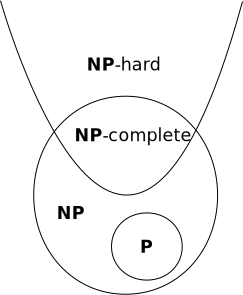
\includegraphics[scale=0.8]{./input/np.pdf}
	\caption{Diagrama das classes de problemas. \label{fig:np}}
\end{figure}

\subsection{Objetivo}

Este trabalho, dentro dos tópicos de Classes de Complexidade (\textit{Complexity Classes}) da disciplina de Linguagens Formais e Teoria da Computação, consiste em explicar do que se trata o Problema da Soma dos Subconjuntos (\textit{Subset Sum Problem}) e apresentar uma prova de sua \textbf{NP}-\textit{completude}. Por ser um problema conhecido e já estudado, este trabalho é um \textbf{exercício de pesquisa} em que são consultadas referências na literatura e sintetizadas aqui pelo grupo.

Todo material pesquisado para este trabalho encontra-se nos capítulos 34 e 35 do livro \textit{Introduction to Algorithms}~\cite{bib:cormen} sugerido como referência nos \textit{slides} de aula da disciplina.

% inkscape -D -z --file=./input/smooth.svg --export-pdf=./input/smooth.pdf

